\chapter{Modellazione dei Casi d'Uso}

\section{Attori e Casi d'Uso}

\begin{table}[h]
	\centering
	\begin{tblr}{colspec=XX}
		\begin{minipage}[t]{\linewidth}
			\paragraph{Attori primari}
			\begin{itemize}
				\item UtenteRegistrato
				\item Cliente
				\item Farmacista
				\item Direttore
				\item Cliente non registrato
			\end{itemize}
		\end{minipage} &
		\begin{minipage}[t]{\linewidth}
			\paragraph{Attori secondari}
			\begin{itemize}
				\item Farmacista
			\end{itemize}
		\end{minipage} \\
	\end{tblr}
\end{table}

\begin{table}[h]
	\centering
	\begin{tblr}{colspec=XX}
		\begin{minipage}[t]{\linewidth}
			\paragraph{Casi d'uso}
			\begin{enumerate}
				\item VisualizzaCatalogo % RF01, RF06
				\item AggiungiFarmaco % RF02
				\item CercaFarmaco % RF18
				\item ModificaFarmaco % RF03
				\item EliminaFarmaco % RF04
				\item RegistraCliente % RF05
				\item CreaOrdine % RF07, RF09, RF17
				\item GeneraOrdineAcquisto % RF10
				\item VisualizzaOrdiniAcquisto % RF11
				\item RegistraConsegnaOrdineAcquisto % RF12
				\item GeneraReport % RF13
				\item VisualizzaOrdiniFarmacia % RF14
				\item RitiraOrdine % RF15
				\item VisualizzaStoricoOrdini % RF16
				\item GeneraOrdineAcquistoFarmacista % RF19
			\end{enumerate}
		\end{minipage} &
		\begin{minipage}[t]{\linewidth}
			\paragraph{Casi d'uso di inclusione}
			\begin{enumerate}
				\item CercaFarmaco
				\item VisualizzaOrdiniFarmacia
				\item VisualizzaOrdiniAcquisto
			\end{enumerate}

			\paragraph{Casi d'uso di estensione}
			\begin{enumerate}
				\item GeneraOrdineAcquisto % RF10
			\end{enumerate}
		\end{minipage}
	\end{tblr}
\end{table}

\begin{table}[!hbp]
	\centering
	\begin{tblr}{
		colspec = lllll,
		hlines,
		row{1} = {font=\bfseries}
	}
		Caso d'uso & Attori primari & {Attori \\ secondari} & Incl. / Ext. & Requisito \\
		VisualizzaCatalogo & UtenteRegistrato & - & - & {\Req{rf}{01} \\ \Req{rf}{06}} \\
		AggiungiFarmaco & Farmacista & - & - & \Req{rf}{02} \\
		CercaFarmaco & UtenteRegistrato & - & - & \Req{rf}{18} \\
		ModificaFarmaco & Farmacista & - & {Include \\ CercaFarmaco} & \Req{rf}{03} \\
		EliminaFarmaco & Farmacista & - & {Include \\ CercaFarmaco} & \Req{rf}{04} \\
		RegistraCliente & {Cliente \\ non registrato} & - & - & \Req{rf}{05} \\
		CreaOrdine & Cliente & - & {Include \\ CercaFarmaco} & {\Req{rf}{07} \\ \Req{rf}{09} \\ \Req{rf}{17}} \\
		GeneraOrdineAcquisto & Cliente & - & Incluso in CreaOrdine & \Req{rf}{10} \\
		VisualizzaOrdiniAcquisto & Farmacista & - & - & \Req{rf}{11} \\
		RegistraConsegnaOrdineAcquisto & Farmacista & - & {Include \\ VisualizzaOrdiniAcquisto} & \Req{rf}{12} \\
		GeneraReport & Direttore & - & - & \Req{rf}{13} \\
		VisualizzaOrdiniFarmacia & Farmacista & - & - & \Req{rf}{14} \\
		RitiraOrdine & Cliente & Farmacista & {Include \\ VisualizzaOrdiniFarmacia} & \Req{rf}{15} \\
		VisualizzaStoricoOrdini & Cliente & - & - & \Req{rf}{16} \\
		GeneraOrdineAcquistoFarmacista & Farmacista & - & - & \Req{rf}{18}
	\end{tblr}
\end{table}

\section{Diagramma dei Casi d'Uso}
% TODO: add image from vpp or create diagram with tikzuml package
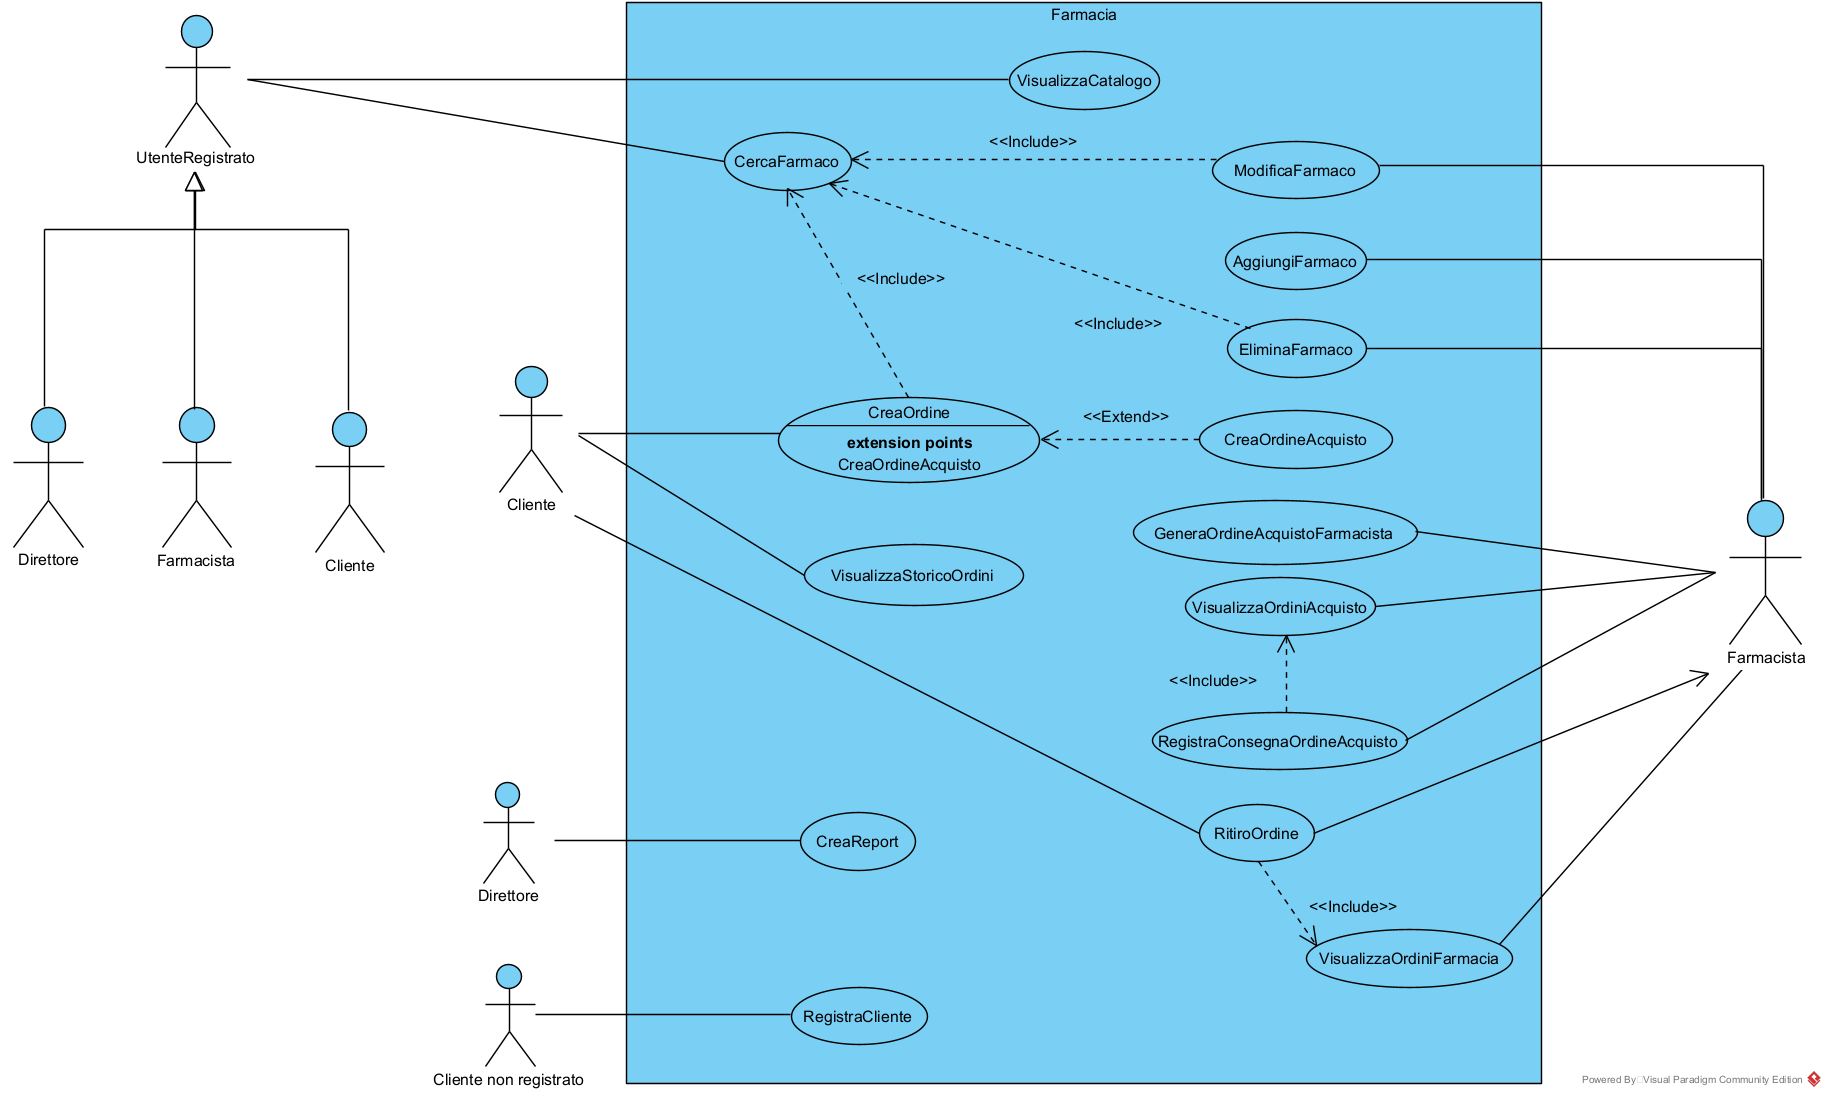
\includegraphics[width=\linewidth]{chapters/usecases/UseCaseFarmacia}
\section{Scenari}

\section{RegistraCliente}

\subsubsection*{Category Partition Testing}

\begin{table}[!hbp]
	\centering
	\footnotesize
	\begin{partest}{colspec = XXXXXX}
		Nome & Cognome & Username & Password & Email & DataNascita \\
		\begin{itemize}[leftmargin=*]
			\item Stringa di lunghezza $\leq$ 45
			\item Stringa di lunghezza $>$ 45 \texttt{[ERROR]}
			\item Stringa vuota \texttt{[ERROR]}
		\end{itemize} &
		\begin{itemize}[leftmargin=*]
			\item Stringa di lunghezza $\leq$ 45
			\item Stringa di lunghezza $>$ 45 \texttt{[ERROR]}
			\item Stringa vuota \texttt{[ERROR]}
		\end{itemize} &
		\begin{itemize}[leftmargin=*]
			\item Stringa di lunghezza $\leq$ 45
			\item Stringa di lunghezza $>$ 45 \texttt{[ERROR]}
			\item Stringa vuota \texttt{[ERROR]}
			\item Stringa già presente nel sistema \texttt{[ERROR]}
		\end{itemize} &
		\begin{itemize}[leftmargin=*]
			\item Stringa di lunghezza compresa tra 8 e 45
			\item Stringa di lunghezza $<$ 8 \texttt{[ERROR]}
			\item Stringa di lunghezza $>$ 45 \texttt{[ERROR]}
		\end{itemize} &
		\begin{itemize}[leftmargin=*]
			\item Stringa di lunghezza $\leq$ 45
			\item Stringa di lunghezza $>$ 45 \texttt{[ERROR]}
			\item Stringa vuota \texttt{[ERROR]}
			\item Stringa già presente nel sistema \texttt{[ERROR]}
		\end{itemize} &
		\begin{itemize}[leftmargin=*]
			\item Data con formato valido (gg-mm-aaaa)
			\item Data con formato non valido \texttt{[ERROR]}
		\end{itemize}
	\end{partest}
\end{table}

\noindent Il numero di test da effettuarsi senza particolari vincoli è: $3 \cdot 3 \cdot 4 \cdot 3 \cdot 4 \cdot 2 = 864$.

\noindent Introduciamo i vincoli \texttt{[ERROR]}. Il numero di test da eseguire per testare singolarmente i vincoli è 13 (2 per Nome, 2 per Cognome, 3 per Username, 2 per Password, 3 per Email, 1 per DataNascita).

\noindent Il numero di test risultante è 14: $(1 \cdot 1 \cdot 1 \cdot 1 \cdot 1 \cdot 1) + 13 = 14$.

\subsubsection*{Test Suite}

\begin{table}[!hbp]
	\centering
	\footnotesize
	\begin{testsuite}{colspec = lXXXlXX}
		{Test \\ Case \\ ID} & Descrizione & Classi di Equivalenza Coperte & Pre-condizioni & Input & {Output \\ Attesi} & {Post-condizioni \\ Attese} \\
		1 & Tutti gli input validi & Nome, Cognome, Username, Password, Email, DataNascita validi & Il cliente non è ancora registrato nel sistema & {Nome: Mario \\ Cognome: Rossi \\ Username: mariorossi \\ Password: miapassword \\ Email: mario@gmail.com \\ DataNascita: 22-06-1989} & Registrazione effettuata & Il cliente è stato correttamente registrato nel sistema \\
		2 & Nome $>$ 45 caratteri & Nome $>$ 45 caratteri \texttt{[ERROR]}, Cognome, Username, Password, Email, DataNascita validi & -- & {Nome: \dots \\ Cognome: Rossi \\ Username: mariorossi \\ Password: miapassword \\ Email: mario@gmail.com \\ DataNascita: 22-06-1989} & Nome troppo lungo & -- \\
		3 & Nome non specificato & Nome non specificato \texttt{[ERROR]}, Cognome, Username, Password, Email, DataNascita validi & -- & {Nome: \\ Cognome: Rossi \\ Username: mariorossi \\ Password: miapassword \\ Email: mario@gmail.com \\ DataNascita: 22-06-1989} & Inserire un nome & -- \\
	\end{testsuite}
\end{table}

\begin{table}[!ht]
	\centering
	\footnotesize
	\begin{testsuite}{colspec = lXXXlXl}
		{Test \\ Case \\ ID} & Descrizione & Classi di Equivalenza Coperte & Pre-condizioni & Input & {Output \\ Attesi} & {Post-\\condizioni \\ Attese} \\
		4 & Cognome $>$ 45 caratteri & Cognome $>$ 45 caratteri \texttt{[ERROR]}, Nome, Username, Password, Email, DataNascita validi & -- & {Nome: Mario \\ Cognome: \dots \\ Username: mariorossi \\ Password: miapassword \\ Email: mario@gmail.com \\ DataNascita: 22-06-1989} & Cognome troppo lungo & -- \\
		5 & Cognome non specificato & Cognome non specificato \texttt{[ERROR]}, Nome, Username, Password, Email, DataNascita validi & -- & {Nome: Mario \\ Cognome: \\ Username: mariorossi \\ Password: miapassword \\ Email: mario@gmail.com \\ DataNascita: 22-06-1989} & Inserire un cognome & -- \\
		6 & Username $>$ 45 caratteri & Username $>$ 45 caratteri \texttt{[ERROR]}, Nome, Cognome, Password, Email, DataNascita validi & -- & {Nome: Mario \\ Cognome: Rossi \\ Username: \dots \\ Password: miapassword \\ Email: mario@gmail.com \\ DataNascita: 22-06-1989} & Username troppo lungo & -- \\
		7 & Username non specificato & Username non specificato \texttt{[ERROR]}, Nome, Cognome, Password, Email, DataNascita validi & -- & {Nome: Mario \\ Cognome: Rossi \\ Username: \\ Password: miapassword \\ Email: mario@gmail.com \\ DataNascita: 22-06-1989} & Inserire uno username & -- \\
		8 & Password $<$ 8 caratteri & Password $<$ 8 caratteri \texttt{[ERROR]}, Nome, Cognome, Username, Email, DataNascita validi & -- & {Nome: Mario \\ Cognome: Rossi \\ Username: mariorossi \\ Password: prova \\ Email: mario@gmail.com \\ DataNascita: 22-06-1989} & Password troppo corta & -- \\
		9 & Password $>$ 45 caratteri & Password $>$ 45 caratteri \texttt{[ERROR]}, Nome, Cognome, Username, Email, DataNascita validi & -- & {Nome: Mario \\ Cognome: Rossi \\ Username: mariorossi \\ Password: \dots \\ Email: mario@gmail.com \\ DataNascita: 22-06-1989} & Password troppo lunga & -- \\
		10 & Email $>$ 45 caratteri & Email $>$ 45 caratteri \texttt{[ERROR]}, Nome, Cognome, Username, Password, DataNascita validi & -- & {Nome: Mario \\ Cognome: Rossi \\ Username: mariorossi \\ Password: miapassword \\ Email: \dots \\ DataNascita: 22-06-1989} & Email troppo lunga & -- \\
		11 & Email non specificato & Email non specificato \texttt{[ERROR]}, Nome, Cognome, Username, Password, DataNascita validi & -- & {Nome: Mario \\ Cognome: Rossi \\ Username: \\ Password: miapassword \\ Email: \\ DataNascita: 22-06-1989} & Inserire un'email & -- \\
		12 & Formato DataNascita non valido & Formato DataNascita non valido \texttt{[ERROR]}, Nome, Cognome, Username, Password, Email validi & -- & {Nome: Mario \\ Cognome: Rossi \\ Username: mariorossi \\ Password: miapassword \\ Email: mario@gmail.com \\ DataNascita: 1989-06-22} & Formato data non valido & -- \\
	\end{testsuite}
\end{table}

\begin{table}[!ht]
	\centering
	\footnotesize
	\begin{testsuite}{colspec = lXXXlll}
		{Test \\ Case \\ ID} & Descrizione & Classi di Equivalenza Coperte & Pre-condizioni & Input & {Output \\ Attesi} & {Post-\\condizioni \\ Attese} \\
		13 & Username già presente nel sistema & Username già esistente \texttt{[ERROR]}, Nome, Cognome, Password, DataNascita ed Email validi & Username ``pippo2002'' già presente nel sistema & {Nome: Pippo \\ Cognome: Baudo \\ Username: pippo2002 \\ Password: miapassword \\ Email: pippo@gmail.com \\ DataNascita: 1989-06-22} & {Username già \\ utilizzato} & -- \\
		14 & Email già presente nel sistema & Email già esistente \texttt{[ERROR]}, Nome, Cognome, Password, DataNascita e Username validi & Email ``pippo@gmail.com'' già presente nel sistema & {Nome: Pippo \\ Cognome: Baudo \\ Username: pippo2002 \\ Password: miapassword \\ Email: pippo@gmail.com \\ DataNascita: 1989-06-22} & {Email già \\ utilizzata} & -- \\
	\end{testsuite}
\end{table}

\begin{table}[!hbp]
	\centering
	\begin{scenery}{colspec=lX}
		Caso d'uso: & VisualizzaCatalogo \\
		Attore primario & UtenteRegistrato \\
		Attore secondario & Nessuno \\
		Descrizione & Un utente visualizza il catalogo della farmacia \\
		Pre-condizioni & Aver effettuato l'accesso al sistema \\
		{Sequenza di eventi \\ principale} &
			\begin{enumerate}
				\item L'utente richiede al sistema di visualizzare il catalogo
				\item Il sistema mostra il catalogo della farmacia
			\end{enumerate} \\
		Post-condizioni & - \\
		Casi d'uso correlati & Nessuno \\
		{Sequenza di eventi \\ alternativa} & -
	\end{scenery}
\end{table}

\section{AggiungiFarmaco}

\subsubsection*{Category Partition Testing}

\begin{table}[!hbp]
	\centering
	\footnotesize
	\begin{tblr}{
		colspec = XXXl,
		hlines, vlines,
		row{1} = {font=\bfseries},
		measure=vbox, stretch=-1
		}
		Nome & Prezzo & Prescrizione & Scorte \\
		\begin{itemize}[leftmargin=*]
			\item Stringa di lunghezza $\leq$ 45
			\item Stringa di lunghezza $>$ 45 \texttt{[ERROR]}
			\item Stringa vuota \texttt{[ERROR]}
		\end{itemize} &
		\begin{itemize}[leftmargin=*]
			\item Numero reale $>0$ (\euro)
			\item Numero reale $\leq 0$ (\euro) \texttt{[ERROR]}
		\end{itemize} &
		\begin{itemize}[leftmargin=*]
			\item {\texttt{True} (necessaria) / \\ \texttt{False} (non necessaria)}
		\end{itemize} &
		\begin{itemize}[leftmargin=*]
			\item Numero intero $\geq 0 $
			\item Numero intero $<0$ \texttt{[ERROR]}
		\end{itemize}
	\end{tblr}
\end{table}

\noindent Il numero di test da effettuarsi senza particolari vincoli è: $3 \cdot 2 \cdot 1 \cdot 2 = 12$.

\noindent Introduciamo i vincoli \texttt{[ERROR]}. Il numero di test da eseguire per testare singolarmente i vincoli è 4 (2 per Nome, 1 per Prezzo, 1 per Scorte).

\noindent Il numero di test risultante è 5: $(1 \cdot 1 \cdot 1 \cdot 1) + 4 = 5$.

\subsubsection*{Test Suite}

\begin{table}[!hbp]
	\centering
	\footnotesize
	\begin{tblr}{
			colspec = lXXXlXX,
			hlines, vlines,
			row{1} = {font=\bfseries},
			measure=vbox
		}
		{Test \\ Case \\ ID} & Descrizione & Classi di Equivalenza Coperte & Pre-condizioni & Input & {Output \\ Attesi} & {Post-condizioni \\ Attese} \\
		1 &
		Tutti gli input validi &
		Nome, Prezzo, Scorte e Prescrizione (sia \texttt{True} che \texttt{False}) validi &
		Il farmaco non è presente nel sistema &
		{Nome: Rocefin \\ Prezzo: 15.00 \euro \\ Scorte: 60 \\ Prescrizione: \texttt{boolean}} &
		Farmaco aggiunto & Il farmaco viene correttamente aggiunto al catalogo \\
	\end{tblr}
\end{table}

\begin{table}[!ht]
	\centering
	\footnotesize
	\begin{tblr}{
			colspec = lXXXlXX,
			hlines, vlines,
			row{1} = {font=\bfseries},
			measure=vbox
		}
		{Test \\ Case \\ ID} & Descrizione & Classi di Equivalenza Coperte & Pre-condizioni & Input & {Output \\ Attesi} & {Post-condizioni \\ Attese} \\
		2 &
		Nome $>$ 45 caratteri &
		Nome $>$ 45 caratteri \texttt{[ERROR]}, Prezzo, Scorte e Prescrizione (sia \texttt{True} che \texttt{False}) validi &
		-- &
		{Nome: \dots \\ Prezzo: 16.10 \euro \\ Scorte: 23 \\ Prescrizione: \texttt{boolean}} &
		Nome troppo lungo &
		-- \\
		3 &
		Nome assente &
		Nome assente \texttt{[ERROR]}, Prezzo, Scorte e Prescrizione (sia \texttt{True} che \texttt{False}) validi &
		-- &
		{Nome: \\ Prezzo: 9.99 \euro \\ Scorte: 10 \\ Prescrizione: \texttt{boolean}} &
		Inserire un nome &
		-- \\
        4 &
        Prezzo $\leq 0$ (\euro) & Prezzo $\leq 0$ (\euro) \texttt{[ERROR]}, Nome, Scorte e Prescrizione (sia \texttt{True} che \texttt{False}) validi &
        -- & {Nome: Brufen \\ Prezzo: -8.00 \euro \\ Scorte: 200 \\ Prescrizione: \texttt{boolean}} & Inserire un prezzo $> 0$ \euro & -- \\
        5 & Scorte $ < 0$ & Scorte $<0$, Nome, Prezzo e Prescrizione (sia \texttt{True} che \texttt{False}) validi & -
        & {Nome: Macladin \\ Prezzo: 11.50 \euro \\ Scorte: -36 \\ Prescrizione: \texttt{boolean}} & Inserire scorte $ \geq 0 $ & -- \\
	\end{tblr}
\end{table}

\section{CercaFarmaco}

\subsubsection*{Category Partition Testing}

\begin{table}[!hbp]
	\centering
	\footnotesize
	\begin{tblr}{
		colspec = X,
		hlines, vlines,
		row{1} = {font=\bfseries},
		measure=vbox, stretch=-1
		}
		Nome \\
		\begin{itemize}[leftmargin=*]
			\item Stringa di caratteri di lunghezza $\leq$ 45
			\item Stringa di caratteri di lunghezza $>$ 45 \texttt{[ERROR]}
			\item Stringa di caratteri vuota \texttt{[ERROR]}
			\item Nome di un farmaco non presente nel sistema \texttt{[ERROR]}
		\end{itemize}
	\end{tblr}
\end{table}

\noindent Essendo previsto un solo input, il numero di test da effettuarsi è pari a 4.

\subsubsection*{Test Suite}

\begin{table}[!hbp]
	\centering
	\footnotesize
	\begin{tblr}{
			colspec = lXXXlXX,
			hlines, vlines,
			row{1} = {font=\bfseries},
			measure=vbox
		}
		{Test \\ Case \\ ID} & Descrizione & Classi di Equivalenza Coperte & Pre-condizioni & Input & {Output \\ Attesi} & {Post-condizioni \\ Attese} \\
		1 & Nome del farmaco valido & Nome del farmaco valido & Il farmaco è presente nel catalogo & Nome : Tachipirina & Il farmaco viene mostrato a video & - \\
		2 & Nome del farmaco $>$ 45 caratteri & Nome del farmaco $>$ 45 caratteri \texttt{[ERROR]} & - & Nome : ... & Nome del farmaco troppo lungo & - \\
		3 & Nome del farmaco assente & Nome del farmaco assente \texttt{[ERROR]} & - & Nome : & Inserire il nome di un farmaco & - \\
		4 & Nome di un farmaco che non esiste & Nome di un farmaco che non esiste \texttt{[ERROR]} & Il farmaco con nome "Tachipirina" non esiste & Nome : Tachipirina & Il farmaco non esiste & - \\
	\end{tblr}
\end{table}
\begin{table}[!hbp]
	\centering
	\footnotesize
	\begin{tblr}{
			colspec = lXXXXX,
			hlines, vlines,
			row{1} = {font=\bfseries},
			measure=vbox
		}
		{Test \\ Case \\ ID} & Descrizione & {Cammino \\ Coperto} & Pre-condizioni & Input & Esito \\
		1 & Il farmaco è presente nel DB ma non nella collection locale, che risulta vuota & 0-1 & Il farmaco è presente nel DB ma non nella collection locale & -- &
       	Cammino non percorribile: la collection locale è sempre sincronizzata con il DB \\
		2 & La collection locale ha un solo farmaco che non è quello da modificare & 0-1-2-4-1 & -- & -- & Cammino non percorribile: se il farmaco è presente nel DB, deve essere presente anche nella collection locale \\
		3 & Il farmaco esiste & 0-1-2-3-4-1 & Il farmaco esiste & {Nome: Plasil \\ Prezzo: 11.50 \euro \\ Scorte: 30 \\ Prescrizione: \texttt{True}} & Farmaco modificato \\
	\end{tblr}
\end{table}
\section{EliminaFarmaco}

\subsubsection*{Category Partition Testing}

\begin{table}[!hbp]
	\centering
	\footnotesize
	\begin{partest}{colspec = X}
		Nome \\
		\begin{itemize}[leftmargin=*]
			\item Stringa di lunghezza $\leq$ 45
			\item Stringa di lunghezza $>$ 45 \texttt{[ERROR]}
			\item Stringa vuota \texttt{[ERROR]}
			\item Stringa non presente nel sistema \texttt{[ERROR]}
		\end{itemize}
	\end{partest}
\end{table}

\noindent Essendo previsto un solo input, il numero di test da effettuarsi è pari a 4.

\subsubsection*{Test Suite}

\begin{table}[!ht]
	\centering
	\footnotesize
	\begin{testsuite}{colspec = lXXXlXX}
		{Test \\ Case \\ ID} & Descrizione & Classi di Equivalenza Coperte & Pre-condizioni & Input & {Output \\ Attesi} & {Post-condizioni \\ Attese} \\
		1 & Nome del farmaco valido & Nome del farmaco valido & Il farmaco è presente nel catalogo & Nome: Tachipirina & Farmaco cancellato & Il farmaco viene cancellato dal catalogo \\
		2 & Nome del farmaco $>$ 45 caratteri & Nome del farmaco $>$ 45 caratteri \texttt{[ERROR]} & -- & Nome: \dots & Nome del farmaco troppo lungo & -- \\
		3 & Nome del farmaco non specificato & Nome del farmaco non specificato \texttt{[ERROR]} & -- & Nome: & Inserire il nome di un farmaco & -- \\
		4 & Il farmaco non esiste & Farmaco non presente nel sistema \texttt{[ERROR]} & Non esiste il farmaco chiamato ``Tachipirina'' & Nome: Tachipirina & Non puoi eliminare un farmaco che non esiste & -- \\
	\end{testsuite}
\end{table}

\begin{table}[!hbp]
	\centering
	\begin{scenery}{colspec=lX}
		Caso d'uso: & VisualizzaOrdiniAcquisto \\
		Attore primario & Farmacista \\
		Attore secondario & Nessuno \\
		Descrizione & Un farmacista visualizza l'elenco degli ordini d'acquisto della farmacia \\
		Pre-condizioni & -- \\
		{Sequenza di eventi \\ principale} &
			\begin{enumerate}
				\item Il farmacista richiede al sistema di visualizzare gli ordini d'acquisto
				\item Il sistema mostra l'elenco degli ordini d'acquisto
			\end{enumerate} \\
		Post-condizioni & L'elenco degli ordini di acquisto è stato mostrato a video \\
		Casi d'uso correlati & Nessuno \\
		{Sequenza di eventi \\ alternativa} & --
	\end{scenery}
\end{table}

\section{RegistraConsegnaOrdineAcquisto}

\subsubsection*{Category Partition Testing}

\begin{table}[!hbp]
	\centering
	\footnotesize
	\begin{partest}{colspec = X}
		Id dell'ordine di acquisto \\
		\begin{itemize}[leftmargin=*]
			\item Stringa di lunghezza $\leq$ 45
			\item Stringa di lunghezza $>$ 45 \texttt{[ERROR]}
			\item Stringa vuota \texttt{[ERROR]}
			\item Stringa non presente nel sistema \texttt{[ERROR]}
		\end{itemize}
	\end{partest}
\end{table}

\noindent Essendo previsto un solo input, il numero di test da effettuarsi è pari a 4.

\subsubsection*{Test Suite}

\begin{table}[!hbp]
	\centering
	\footnotesize
	\begin{testsuite}{colspec = lXXXXXX}
		{Test \\ Case \\ ID} & Descrizione & Classi di Equivalenza Coperte & Pre-condizioni & Input & {Output \\ Attesi} & {Post-condizioni \\ Attese} \\
		1 & Id dell'ordine di acquisto valido & Id dell'ordine di acquisto valido & -- & {Id: 5ea930bc-f0a5-427a-8ca1-f9a2a6146948} & Ordine ricevuto & Lo stato dell'ordine di acquisto e le scorte in magazzino sono aggiornati \\
		2 & Id $>$ 45 caratteri & Id $>$ 45 caratteri \texttt{[ERROR]} & -- & Id: \dots & Id troppo lungo & -- \\
		3 & Id vuoto & Id vuoto \texttt{[ERROR]} & -- & Id: & Inserire l'Id di un ordine di acquisto & -- \\
		4 & Id inesistente & Id inesistente \texttt{[ERROR]} & Non esiste un ordine di acquisto con Id ``5ea930bc-f0a5-427a-8ca1-f9a2a6146948'' & Id: 5ea930bc-f0a5-427a-8ca1-f9a2a6146948 & L'ordine di acquisto non esiste & -- \\
	\end{testsuite}
\end{table}

\begin{table}[!hbp]
	\centering
	\begin{scenery}{colspec=lX}
		Caso d'uso: & VisualizzaOrdiniFarmacia \\
		Attore primario & Farmacista \\
		Attore secondario & Nessuno \\
		Descrizione & Un farmacista visualizza l'elenco degli ordini effettuati dai clienti \\
		Pre-condizioni & -- \\
		{Sequenza di eventi \\ principale} &
			\begin{enumerate}
				\item Il farmacista richiede al sistema di visualizzare gli ordini dei clienti
				\item Il sistema mostra l'elenco degli ordini dei clienti
			\end{enumerate} \\
		Post-condizioni & L'elenco degli ordini dei clienti è mostrato a video \\
		Casi d'uso correlati & Nessuno \\
		{Sequenza di eventi \\ alternativa} & --
	\end{scenery}
\end{table}

\begin{table}[!hbp]
	\centering
	\begin{scenery}{colspec=lX}
		Caso d'uso: & RitiraOrdine \\
		Attore primario & Cliente \\
		Attore secondario & Farmacista \\
		Descrizione & Un cliente ritira l'ordine effettuato online \\
		Pre-condizioni & Esiste l'ordine nel sistema \\
		{Sequenza di eventi \\ principale} &
			\begin{enumerate}
				\item Il cliente arriva in farmacia e richiede il ritiro di un ordine mostrando la ricevuta
				\item \textit{include} (VisualizzaOrdiniFarmacia)
				\item Il farmacista seleziona l'ordine di interesse
				\item Il farmacista richiede al sistema di modificare lo stato dell'ordine
			\end{enumerate} \\
		Post-condizioni & Lo stato dell'ordine è stato correttamente modificato \\
		Casi d'uso correlati & Nessuno \\
		{Sequenza di eventi \\ alternativa} & --
	\end{scenery}
\end{table}

\begin{table}[!hbp]
	\centering
	\begin{scenery}{colspec=lX}
		Caso d'uso: & VisualizzaStoricoOrdini \\
		Attore primario & Cliente \\
		Attore secondario & -- \\
		Descrizione & Un cliente visualizza lo storico dei suoi ordini \\
		Pre-condizioni & Il cliente è autenticato \\
		{Sequenza di eventi \\ principale} &
			\begin{enumerate}
				\item Il cliente richiede al sistema di visualizzare lo storico dei suoi ordini
				\item Il sistema mostra lo storico degli ordini
			\end{enumerate} \\
		Post-condizioni & Viene mostrato lo storico degli ordini del cliente \\
		Casi d'uso correlati & Nessuno \\
		{Sequenza di eventi \\ alternativa} & --
	\end{scenery}
\end{table}

\begin{table}[!hbp]
	\centering
	\begin{scenery}{colspec=lX}
		Caso d'uso: & CreaOrdine \\
		Attore primario & Cliente \\
		Attore secondario & - \\
		Descrizione & Un cliente genera un ordine contenente farmaci presenti in catalogo \\
		Pre-condizioni & Il cliente è autenticato \\
		{Sequenza di eventi \\ principale} &
			\begin{enumerate}
				\item Il cliente richiede al sistema di creare un ordine
				\item Il sistema mostra a video la lista dei farmaci
				\item Finché il cliente vuole aggiungere farmaci all'ordine
				\begin{enumerate}[label*=\arabic*.]
					\item Se viene richiesto un farmaco non da banco, il sistema chiede conferma del possesso della prescrizione
					\item Il cliente seleziona la quantità di farmaco desiderata
					\item Il sistema verifica che le scorte siano sufficienti
					\item Il sistema crea l'ordine con i farmaci inseriti e aggiorna le scorte
					\item \textit{punto di estensione}: GeneraOrdineAcquisto
				\end{enumerate}
				\item Il sistema mostra al cliente il resoconto dell'ordine e l'importo totale
				\item Se il cliente conferma l'acquisto
				\begin{enumerate}[label*=\arabic*.]
					\item Il sistema restituisce una ricevuta al cliente
				\end{enumerate}
				\item Altrimenti
				\begin{enumerate}[label*=\arabic*.]
					\item Il sistema elimina l'ordine
				\end{enumerate}
			\end{enumerate} \\
		Post-condizioni & È stato correttamente generato un ordine \\
		Casi d'uso correlati & Nessuno \\
		{Sequenza di eventi \\ alternativa} &
			\begin{enumerate}
				\item Al punto 3.1, il sistema mostra un messaggio di errore se il cliente non è in possesso della prescrizione
				\begin{enumerate}[label*=\arabic*.]
					\item Il farmaco non viene aggiunto all'ordine, il caso d'uso prosegue al punto 3
				\end{enumerate}
				\item Al punto 3.3, il sistema rileva che le scorte non sono sufficienti
					\begin{enumerate}[label*=\arabic*.]
						\item Il farmaco viene rimosso dall'ordine
					\end{enumerate}
			\end{enumerate} \\
	\end{scenery}
\end{table}

\begin{table}[!hbp]
	\centering
	\begin{scenery}{colspec=lX}
		{Caso d'uso \\ d'estensione}: & GeneraOrdineAcquisto \\
		Attore primario & Cliente \\
		Attore secondario & -- \\
		Descrizione & Il sistema genera un ordine di fornitura \\
		Pre-condizioni & Le scorte di uno o più prodotti sono terminate \\
		{Sequenza di eventi \\ principale} &
			\begin{enumerate}
				\item Per ogni farmaco senza scorte
				\begin{enumerate}[label*=\arabic*.]
					\item Il sistema aggiunge il farmaco all'ordine d'acquisto con una quantità di default
				\end{enumerate}
				\item Il sistema crea l'ordine d'acquisto
			\end{enumerate} \\
		Post-condizioni & Viene generato un nuovo ordine d'acquisto \\
		Casi d'uso correlati & CreaOrdine \\
		{Sequenza di eventi \\ alternativa} & --
	\end{scenery}
\end{table}

\section{GeneraOrdineAcquistoFarmacista}

\begin{table}[H]
	\centering
	\footnotesize
	\begin{partest}{colspec = XXXl}
		Farmaci-Quantità \\
		\begin{itemize}[leftmargin=*]
			\item Lista di coppie (nomeFarmaco, quantità) non vuota. Per ogni nomeFarmaco esiste un corrispondente farmaco nel sistema.
			\item Lista vuota \texttt{[ERROR]}
		\end{itemize}
	\end{partest}
\end{table}

\noindent Essendo previsto un solo input, il numero di test da effettuarsi è pari a 2.

\subsubsection*{Test Suite}

\begin{table}[H]
	\centering
	\footnotesize
	\begin{testsuite}{colspec = lXXXlXX}
		{Test \\ Case \\ ID} & Descrizione & Classi di Equivalenza Coperte & Pre-condizioni & Input & {Output \\ Attesi} & {Post-condizioni \\ Attese} \\
		1 & Ordine valido & Farmaci-Quantità valido & Esistono nel sistema i farmaci 'Tachipirina' e 'Fluifort' & {[('Tachipirina', 5),\\ ('Fluifort', 10)]} & Ordine di acquisto generato & Un ordine di acquisto viene correttamente creato \\
		2 & Ordine vuoto & Lista vuota \texttt{[ERROR]} & -- & -- & Non puoi creare un ordine di acquisto vuoto & -- \\
	\end{testsuite}
\end{table}

\begin{table}[!hbp]
	\centering
	\begin{scenery}{colspec=lX}
		Caso d'uso: & GeneraReport \\
		Attore primario & Direttore \\
		Attore secondario & -- \\
		Descrizione & Il Direttore della farmacia genera un report \\
		Pre-condizioni & -- \\
		{Sequenza di eventi \\ principale} &
			\begin{enumerate}
				\item Il Direttore richiede al sistema di generare un report
				\item Il Direttore inserisce un intervallo di date
				\item Il sistema genera e mostra il report
			\end{enumerate} \\
		Post-condizioni & Viene generato un nuovo report \\
		Casi d'uso correlati & Nessuno \\
		{Sequenza di eventi \\ alternativa} & --
	\end{scenery}
\end{table}

